%%%%%%%%%%%%%%%%%%%%%%%%%%%%%%%%%%%%%%%%%%%%%%%%%%%%%%%%%%%%%%%%%%%%%%%%%%%%%%%%%
\subsection{Low-Order Scheme}
%%%%%%%%%%%%%%%%%%%%%%%%%%%%%%%%%%%%%%%%%%%%%%%%%%%%%%%%%%%%%%%%%%%%%%%%%%%%%%%%%
\begin{frame}
\frametitle{Invariant Domain}

\begin{itemize}
  \item For the \emph{systems} case, discrete maximum principles no longer apply;
    the concept of \hlorange{invariant domains} becomes the desired tool.
  \item The objective is to prove that the solution
    $\approximatevectorsolution^{n+1}\equiv\discreteprocess
      (\approximatevectorsolution^n)$ belongs to an invariant domain with
    respect to the discrete solution process $\discreteprocess$.
  \item First one assumes that the initial data belongs
    to a convex invariant admissible set: $\vectorsolution^0\in\invariantset$.
  \item Next one expresses $\discreteprocess(\approximatevectorsolution^n)$
    as a convex combination of states:
    $\sum_i\convexcoefficient_i\convexelement_i$, and proves the following:
    \begin{enumerate}
      \item $\sum_i \convexcoefficient_i = 1$
      \item $\convexcoefficient_i \geq 0 \quad \forall i$
      \item $\convexelement_i \in \invariantset \quad \forall i$
    \end{enumerate}
  \item Thus it is proven that
    $\discreteprocess(\approximatevectorsolution^n)\in\invariantset$ since
    $\invariantset$ is a convex set, and thus $\invariantset$ is an invariant
    domain for $\discreteprocess$.
\end{itemize}

\end{frame}
%%%%%%%%%%%%%%%%%%%%%%%%%%%%%%%%%%%%%%%%%%%%%%%%%%%%%%%%%%%%%%%%%%%%%%%%%%%%%%%%%
\begin{frame}
\frametitle{Invariant Domain}

\begin{itemize}
  \item \hlorange{Invariant set} definition: A set such that (the entropy solution
    of the Riemann problem
    using any 2 elements in the set as left and right states) remains in the set.
  \item Example: suppose the initial data belongs to the invariant set 
    \[
      \invariantset_{a,b} \equiv \{(\height,\height u) \,|\,
        a \leq w_2(\height, \height u) \eqc \, w_1(\height, \height u) \leq b\} \eqc
    \]
    where $w_1(\vectorsolution)$ and $w_2(\vectorsolution)$ are Riemann invariants.
\end{itemize}

\begin{center}
  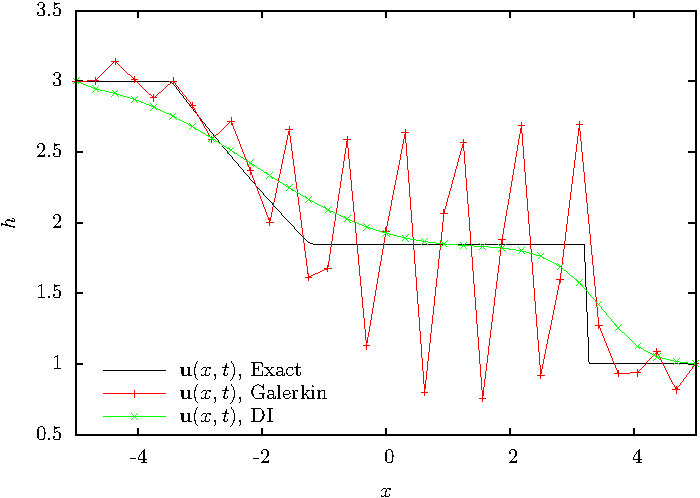
\includegraphics[width=0.45\textwidth]{./figures/dam_break_height.pdf}
  \hspace{1ex}
  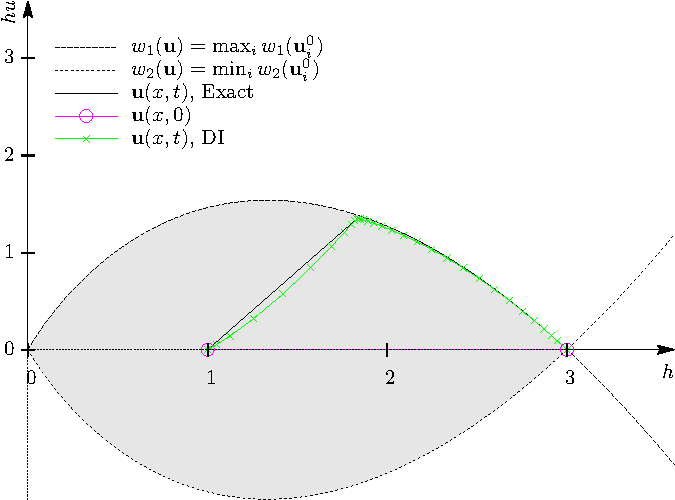
\includegraphics[width=0.45\textwidth]{./figures/dam_break_phase_without_galerkin.pdf}
\end{center}

\end{frame}
%%%%%%%%%%%%%%%%%%%%%%%%%%%%%%%%%%%%%%%%%%%%%%%%%%%%%%%%%%%%%%%%%%%%%%%%%%%%%%%%%
\begin{frame}
\frametitle{Invariant Domain}

\begin{itemize}
  \item \hlorange{Invariant set} definition: A set such that (the entropy solution
    of the Riemann problem
    using any 2 elements in the set as left and right states) remains in the set.
  \item Example: suppose the initial data belongs to the invariant set 
    \[
      \invariantset_{a,b} \equiv \{(\height,\height u) \,|\,
        a \leq w_2(\height, \height u) \eqc \, w_1(\height, \height u) \leq b\} \eqc
    \]
    where $w_1(\vectorsolution)$ and $w_2(\vectorsolution)$ are Riemann invariants.
\end{itemize}

\begin{center}
  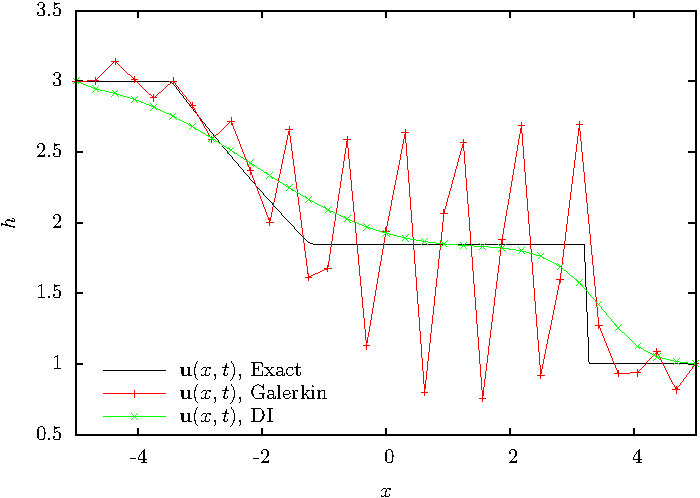
\includegraphics[width=0.45\textwidth]{./figures/dam_break_height.pdf}
  \hspace{1ex}
  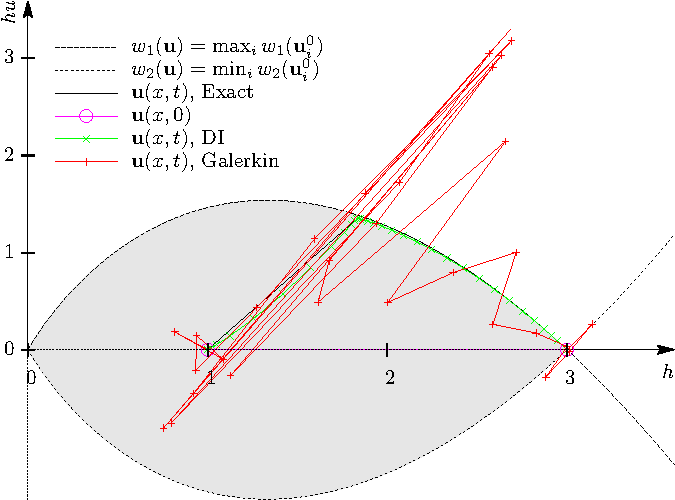
\includegraphics[width=0.45\textwidth]{./figures/dam_break_phase_with_galerkin.pdf}
\end{center}

\end{frame}
%%%%%%%%%%%%%%%%%%%%%%%%%%%%%%%%%%%%%%%%%%%%%%%%%%%%%%%%%%%%%%%%%%%%%%%%%%%%%%%%%
\begin{frame}
\frametitle{Low-Order Scheme}

\begin{itemize}
  \item The domain-invariant low-order scheme lumps the mass matrix and adds
    a low-order diffusion term:
    \begin{equation}
      \textcolor{secondarycolorheavy}{\lumpedmassentry}
        \frac{\solutionvector_i^{L,n+1}-\solutionvector_i^n}{\dt}
        + \sum_j\gradiententry\cdot\consfluxinterpolant_j^n
        + \textcolor{secondarycolorheavy}{
          \sum_j\diffusionmatrixletter\ij^{L,n}\solutionvector_j^n}
        = \ssrhs_i^n \eqc
    \end{equation}
  \item The following definition for the low-order diffusion matrix allows
    the invariant domain property to be proven:
    \begin{equation}
      \diffusionmatrixletter^{L,n}\ij \equiv
        \max(\maxwavespeed\ij\ltwonorm{\mathbf{\gradientmatrixletter}\ij},
          \maxwavespeed\ji\ltwonorm{\mathbf{\gradientmatrixletter}\ji})
      \quad j\ne i \eqc \quad
    \end{equation}
    \begin{equation}
      \diffusionmatrixletter^{L,n}_{i,i} \equiv
        -\sumjnoti\diffusionmatrixletter^{L,n}\ij
      \eqc
    \end{equation}
   where $\maxwavespeed\ij \equiv \maxwavespeed(
   \normalvector\ij,\solutionvector_i^n,\solutionvector_j^n)$
   is the maximum wave speed in the 1-D Riemann problem in the direction
   $\normalvector\ij \equiv \mathbf{\gradientmatrixletter}\ij /
   \ltwonorm{\mathbf{\gradientmatrixletter}\ij}$
   with left state $\solutionvector_i^n$ and right state $\solutionvector_j^n$.
\end{itemize}

\end{frame}
%%%%%%%%%%%%%%%%%%%%%%%%%%%%%%%%%%%%%%%%%%%%%%%%%%%%%%%%%%%%%%%%%%%%%%%%%%%%%%%%%
\begin{frame}
\frametitle{Maximum Wave Speeds}

\begin{itemize}
  \item Consider an example for the 1-D SWE Riemann problem, where the left
    wave is a shock, and the right is a rarefaction:
    \begin{center}
      \begin{tikzpicture}[
  scale=1]

\def\mylength{3}

% axes
\draw[-latex] (0,0) -- (\mylength,0);
\draw[-latex] (0,0) -- (-\mylength,0);
\draw[-latex] (0,0) -- (0,\mylength);
\node at (0.15,\mylength) {$t$};
\node at (\mylength,-0.15) {$x$};

% characteristics
\draw (0,0) -- (30:\mylength);
\draw (0,0) -- (32:\mylength);
\draw (0,0) -- (34:\mylength);
\draw (0,0) -- (36:\mylength);
\draw (0,0) -- (38:\mylength) node[pos=0.5,sloped,above] {2-rarefaction};
\draw (0,0) -- (135:\mylength) node[pos=0.5,sloped,above] {1-shock};
\node at ($(135:\mylength)+(-0.2,0.2)$) {$\lambda_1$};
\node at ($(38:\mylength)+(0.2,0.2)$) {$\lambda_2^-$};
\node at ($(30:\mylength)+(0.25,0.1)$) {$\lambda_2^+$};

% solution values
\node at (155.5:0.75*\mylength) {$\mathbf{u}_L$};
\node at (15:0.75*\mylength) {$\mathbf{u}_R$};
\node at (64:0.75*\mylength) {$\mathbf{u}_*$};

\end{tikzpicture}

    \end{center}
  \item For a general conservation law system of size $m$,
    \begin{equation}
      \maxwavespeed(\vectorsolution_L,\vectorsolution_R)
        = \max\pr{|\lambda_1^-|,|\lambda_m^+|} \eqp
    \end{equation}
  \item Then for the example above
    $\maxwavespeed(\vectorsolution_L,\vectorsolution_R)$ is the maximum of
    the shock speed $|\lambda_1|$ and rarefaction \emph{head} speed $|\lambda_2^+|$.
\end{itemize}

\end{frame}
%%%%%%%%%%%%%%%%%%%%%%%%%%%%%%%%%%%%%%%%%%%%%%%%%%%%%%%%%%%%%%%%%%%%%%%%%%%%%%%%%
\begin{frame}
\frametitle{Maximum Wave Speeds (Cont.)}

\begin{itemize}
  \item For the SWE, a left \textcolor{secondarycolorheavy}{shock} has the wave speed
\begin{equation}\label{eq:left_shockspeed}
  \wavespeed_1^-(\vectorsolution_L, \vectorsolution_R)
    = \velocityx_L - \speedofsound_L\pr{1 + \pr{
    \frac{(\height_* - \height_L)(\height_* + 2\height_L)}{2\height_L^2}}}^{\frac{1}{2}}
    \eqc
\end{equation}
    where $\speedofsound=\sqrt{\gravity\height}$ is the ``speed of sound'' for the SWE.
  \item A left \textcolor{secondarycolorheavy}{rarefaction} has the head wave speed
\begin{equation}\label{eq:leftwavespeed_rarefaction}
  \wavespeed_1^-(\vectorsolution_L, \vectorsolution_R)
    = \velocityx_L - \speedofsound_L
    \eqc
\end{equation}
  \item Note the shock speed depends on the intermediate (star-state) solution
    for height $\height_*$, which may be computed with the following steps:
    \begin{itemize}
      \item Apply Rankine-Hugoniot condition to shock(s)
      \item Apply Riemann invariant condition to rarefaction(s)
      \item Combine resulting expressions and solve nonlinear equation for
        $\height_*$
    \end{itemize}
\end{itemize}

\end{frame}
